% Gestion du temps
\section{Gestion du temps}

\begin{figure}[h] 
    \centering
    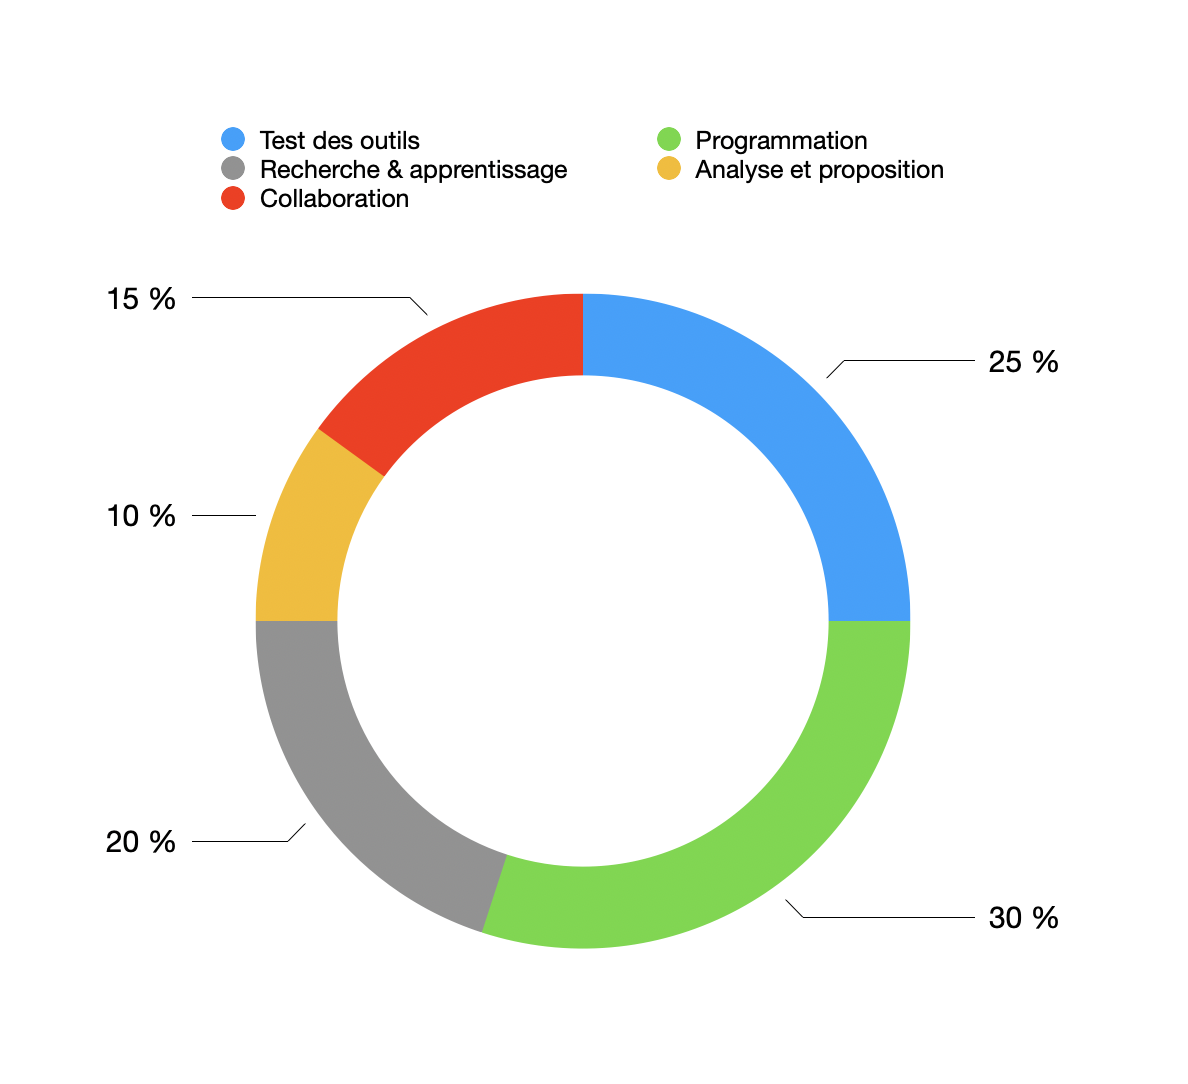
\includegraphics[width=0.7\textwidth]{Includes/Images/gestionTemps.png}
    \caption{Diagramme circulaire - Gestion du temps}
    \label{fig:Diagramme circulaire - Gestion du temps}
\end{figure}  

Pendant mon stage, j'ai accordé une grande importance à une gestion efficace du temps, afin de maximiser ma productivité et de mener à bien les différentes tâches qui m'ont été confiées. Voici une vue d'ensemble de ma gestion du temps (figure \ref{fig:Diagramme circulaire - Gestion du temps}), basée sur les pourcentages suivants :

\begin{itemize}
\item \textbf{Programmation} : J'ai consacré environ 30\% de mon temps à la programmation. Cela inclut la création le développement en React et Next.js pour créer le prototype de la solution avec la connexion avec le Headless CMS et la mise en place du motif de conception.

\item \textbf{Test des outils} : Environ 25\% de mon temps a été dédié aux tests des outils. J'ai testé les outils Relume, Webflow et Devlink pour voir s'ils répondaient aux besoins du projet et pour identifier les avantages et les inconvénients de chacun.

\item \textbf{Recherche et apprentissage} : Environ 20\% de mon temps a été consacré à la recherche et à l'apprentissage de nouvelles technologies et des nouveaux outils. J'ai appris à utiliser des outils tels que Webflow, Relume et ContentFul pour le headless CMS, et j'ai approfondi mes connaissances en Next.js 14 qui a apporté des changements et nouvelles fonctionnalités.
\\ \\
\vspace*{1cm}
\item \textbf{Collaboration} : J'ai consacré environ 15\% de mon temps à la collaboration avec l'équipe autour du projet. Cela comprenait des réunions, des discussions et des échanges d'idées pour garantir que le projet prenne la bonne direction, la prise en compte des éventuelles suggestions et la validation de l'avancée de projet.

\item \textbf{Analyse et proposition}: Environ 10\% de mon temps a été consacré à l'analyse des spécifications ; à la proposition de solutions adaptées aux besoins du projet et du cahier des charges. Cette phase m'a permis de comprendre en détail les exigences et d'identifier les meilleures approches pour les satisfaire.
\end{itemize}

De ce fait, cette gestion du temps équilibrée m'a permis de mener à bien mes tâches et d'atteindre les objectifs fixés dans les délais impartis. Cette répartition réfléchie du temps m'a permis de rester organisé, de faire face aux défis et d'obtenir des résultats positifs tout au long de mon stage.

\subsection*{Communication et gestion de projets}

Pendant les quatres mois de mon stage, nous avons mis en place une solide gestion de projet, qui nous a permis de progresser de manière efficace et de répondre aux attentes fixées. Dès le début, j’ai reçu le cahier des charges détaillant les objectifs et les exigences du projet. Cela m’a donné une vision claire de ce qui était attendu et j’ai pu commencer à développer en conséquence.

Pour assurer un suivi régulier et des retours constructifs, j’ai adopté une approche itérative dans mon travail. À chaque petite étape ou module que je complétais, je les soumettais à M. Marc Raffalli, mon mentor et developpeur front-end senior. Il examinait attentivement mon travail et me fournissait des retours précieux. J’ai pris en compte ces commentaires et suggestions, ce qui m’a permis d’améliorer continuellement mes réalisations avant de passer à l’étape suivante.
\\ \\
Cette méthodologie agile a permis une flexibilité accrue, une adaptation en temps réel aux changements et une amélioration constante tout au long du processus de développement.
